\documentclass[11pt]{article}
\usepackage{cornell-notes}
\usepackage{mathtools}
\usepackage{needspace}
\usepackage{ragged2e}
\usepackage{adjustbox}
\usepackage{tikz}
\usetikzlibrary{arrows.meta,positioning}
\tcbuselibrary{most}
\geometry{letterpaper,margin=0.72in,headheight=15pt}
\setCornellCollection{Calculus Cornell Notes}
\setCornellUnitType{Chapter}
\setCornellUnitNumber{P}
\setCornellUnitTitle{Preparation for Calculus}

\definecolor{Ink}{HTML}{17324D}
\definecolor{Teal}{HTML}{147D78}
\definecolor{Sky}{HTML}{DDEEF1}
\definecolor{Cue}{HTML}{EEF2F5}
\definecolor{Warm}{HTML}{FFF3D6}
\definecolor{Alert}{HTML}{9D3C32}
\definecolor{Green}{HTML}{276749}
\definecolor{Rule}{HTML}{AAB8C2}
\hypersetup{colorlinks=true,linkcolor=Ink,urlcolor=Teal,pdfborder={0 0 0}}
\setlength{\parindent}{0pt}
\setlength{\parskip}{4pt}
\setlist{nosep,leftmargin=*}
\titleformat{\section}{\Large\bfseries\color{Ink}}{}{0pt}{}[\color{Teal}\titlerule]
\titleformat{\subsection}{\large\bfseries\color{Teal}}{}{0pt}{}
\pagestyle{fancy}
\fancyhf{}
\fancyhead[L]{\small\color{Ink}\textsc{Cornell Notes}}
\fancyhead[R]{\small\color{Teal}\nouppercase{\leftmark}}
\fancyfoot[L]{\footnotesize\color{Ink}Active recall $\bullet$ Worked reasoning $\bullet$ Verification}
\fancyfoot[R]{\footnotesize\color{Ink}\thepage\ of \pageref*{LastPage}}
\renewcommand{\headrulewidth}{0.5pt}
\renewcommand{\footrulewidth}{0.4pt}
\newcolumntype{Y}{>{\RaggedRight\arraybackslash}X}
\newtcolorbox{orientationbox}{enhanced,breakable,colback=Sky,colframe=Teal,boxrule=0.7pt,arc=2mm,title=Chapter orientation,fonttitle=\bfseries}
\newtcolorbox{sectionsummarybox}{enhanced,breakable,colback=white,colframe=Teal,boxrule=0.6pt,arc=1.5mm,left=2mm,right=2mm,top=1mm,bottom=1mm,title=Section synthesis,fonttitle=\bfseries\color{Teal}}
\newtcolorbox{warningbox}{enhanced,breakable,colback=Warm,colframe=Alert,boxrule=0.7pt,arc=1.5mm,title=Common error audit,fonttitle=\bfseries}
\newtcolorbox{checkbox}{enhanced,breakable,colback=white,colframe=Green,boxrule=0.7pt,arc=1.5mm,title=Verification habit,fonttitle=\bfseries}
\newcommand{\cornellcuehead}{\rowcolor{Ink}\color{white}\bfseries Cue / recall prompt & \color{white}\bfseries Notes / reasoning \\\endhead}
\newcommand{\cornellcuerow}[2]{\rowcolor{Cue}#1 & #2 \\\addlinespace[3pt]}
% Table-safe: delegates to the shared Cornell formula box (cornell-notes.sty),
% which cannot emit \pagebreak/\noalign inside longtable cells.
\newcommand{\formula}[1]{\CornellFormula[colback=Sky,colframe=Teal]{#1}}

\title{Preparation: Preparation for Calculus\\[2mm]\large Cornell Notes}
\author{}
\date{}
\hypersetup{pdftitle={Preparation: Preparation for Calculus - Cornell Notes},pdfauthor={},pdfsubject={Calculus study notes},pdfkeywords={calculus, Cornell notes, active recall}}
\begin{document}
\maketitle
\thispagestyle{fancy}
\begin{orientationbox}
Build the algebraic, graphical, functional, and trigonometric fluency that later limit, derivative, and integral arguments assume. These notes follow the complete local section sequence (1--44) and emphasize definitions, governing results, strategy selection, and verifiable reasoning.
\end{orientationbox}

\section{Prerequisite map}
\begin{minipage}[t]{0.42\textwidth}
\textbf{Bring forward}
\begin{itemize}
\item Algebraic manipulation
\item Coordinate geometry
\item Function notation
\item Right-triangle trigonometry
\end{itemize}
\end{minipage}\hfill
\begin{minipage}[t]{0.54\textwidth}
\textbf{Chapter flow}
\begin{center}
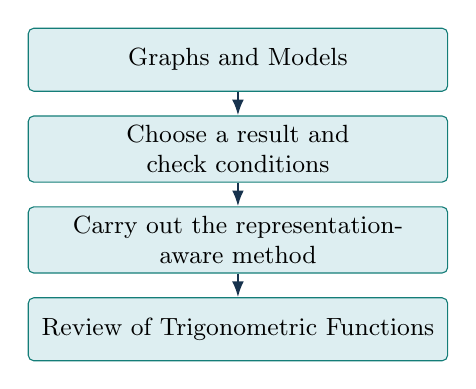
\begin{tikzpicture}[node distance=3mm, every node/.style={font=\small,align=center}, box/.style={draw=Teal,rounded corners=2pt,fill=Sky,minimum height=8mm,text width=0.42\textwidth}, arr/.style={-{Latex[length=2mm]},thick,draw=Ink}]
\node[box] (a) {Graphs and Models};
\node[box,below=of a] (b) {Choose a result and check conditions};
\node[box,below=of b] (c) {Carry out the representation-aware method};
\node[box,below=of c] (d) {Review of Trigonometric Functions};
\draw[arr] (a)--(b); \draw[arr] (b)--(c); \draw[arr] (c)--(d);
\end{tikzpicture}
\end{center}
\end{minipage}

\section{Learning objectives}
\begin{enumerate}
\item Explain the central objects and hypotheses in P.1 and P.4.
\item Translate among algebraic, graphical, numerical, and verbal representations.
\item Select an appropriate formula or theorem before beginning symbolic work.
\item Carry out multi-step calculations while preserving domain, sign, orientation, and units.
\item Diagnose common errors by testing assumptions and checking the result independently.
\item Synthesize the chapter's methods into a reusable problem-solving workflow.
\end{enumerate}

\section{P.1 Graphs and Models}
\begin{longtable}{C N}\cornellcuehead
\cornellcuerow{What is the governing idea in P.1?}{A graph encodes how two quantities vary, while a mathematical model connects that representation to a stated context and domain.}
\cornellcuerow{Which result should be recalled?}{\formula{m=\frac{y_2-y_1}{x_2-x_1}}}
\cornellcuerow{How should a problem be organized?}{Identify variables and units, choose a viewing window, locate intercepts and symmetry, and interpret changes in the context of the model.}
\cornellcuerow{What should be checked before accepting an answer?}{Confirm the hypotheses and domain, preserve units and orientation when relevant, and substitute or differentiate back into the defining relation.}
\end{longtable}
\begin{warningbox}A convincing plot can conceal an inappropriate domain, a distorted scale, or behavior outside the data range.\end{warningbox}
\begin{sectionsummarybox}A graph encodes how two quantities vary, while a mathematical model connects that representation to a stated context and domain. The operational habit is to identify variables and units, choose a viewing window, locate intercepts and symmetry, and interpret changes in the context of the model.\end{sectionsummarybox}
\section{P.2 Linear Models and Rates of Change}
\begin{longtable}{C N}\cornellcuehead
\cornellcuerow{What is the governing idea in P.2?}{A linear model has constant rate of change; slope measures output change per unit input change.}
\cornellcuerow{Which result should be recalled?}{\formula{y-y_1=m(x-x_1),\qquad m=\frac{\Delta y}{\Delta x}}}
\cornellcuerow{How should a problem be organized?}{Compute slope with units, choose a line form, solve for the requested quantity, and decide whether interpolation or extrapolation is being used.}
\cornellcuerow{What should be checked before accepting an answer?}{Confirm the hypotheses and domain, preserve units and orientation when relevant, and substitute or differentiate back into the defining relation.}
\end{longtable}
\begin{warningbox}Reversing the order in only one difference changes the sign; extrapolation may also exceed the model's credible range.\end{warningbox}
\begin{sectionsummarybox}A linear model has constant rate of change; slope measures output change per unit input change. The operational habit is to compute slope with units, choose a line form, solve for the requested quantity, and decide whether interpolation or extrapolation is being used.\end{sectionsummarybox}
\section{P.3 Functions and Their Graphs}
\begin{longtable}{C N}\cornellcuehead
\cornellcuerow{What is the governing idea in P.3?}{A function assigns exactly one output to each input in its domain; transformations and combinations build new functions from known ones.}
\cornellcuerow{Which result should be recalled?}{\formula{(f\circ g)(x)=f(g(x)),\qquad f^{-1}(f(x))=x}}
\cornellcuerow{How should a problem be organized?}{State the domain first, evaluate compositions from the inside out, and track how shifts, reflections, and scalings move key points.}
\cornellcuerow{What should be checked before accepting an answer?}{Confirm the hypotheses and domain, preserve units and orientation when relevant, and substitute or differentiate back into the defining relation.}
\end{longtable}
\begin{warningbox}An inverse relation is a function only when the original function is one-to-one on the chosen domain.\end{warningbox}
\begin{sectionsummarybox}A function assigns exactly one output to each input in its domain; transformations and combinations build new functions from known ones. The operational habit is to state the domain first, evaluate compositions from the inside out, and track how shifts, reflections, and scalings move key points.\end{sectionsummarybox}
\section{P.4 Review of Trigonometric Functions}
\begin{longtable}{C N}\cornellcuehead
\cornellcuerow{What is the governing idea in P.4?}{Trigonometric functions connect angles, unit-circle coordinates, periodic behavior, and geometric ratios.}
\cornellcuerow{Which result should be recalled?}{\formula{\sin^2 x+\cos^2 x=1,\qquad 1+\tan^2x=\sec^2x}}
\cornellcuerow{How should a problem be organized?}{Convert angle units when required, use the unit circle for signs and exact values, then apply identities without changing the expression's domain.}
\cornellcuerow{What should be checked before accepting an answer?}{Confirm the hypotheses and domain, preserve units and orientation when relevant, and substitute or differentiate back into the defining relation.}
\end{longtable}
\begin{warningbox}Degree mode, quadrant errors, and division by a possibly zero trigonometric expression invalidate otherwise sound algebra.\end{warningbox}
\begin{sectionsummarybox}Trigonometric functions connect angles, unit-circle coordinates, periodic behavior, and geometric ratios. The operational habit is to convert angle units when required, use the unit circle for signs and exact values, then apply identities without changing the expression's domain.\end{sectionsummarybox}

\section{Definitions and theorem register}
\small
\begin{longtable}{@{}>{\RaggedRight\arraybackslash}p{0.24\textwidth}>{\RaggedRight\arraybackslash}p{0.40\textwidth}>{\RaggedRight\arraybackslash}p{0.29\textwidth}@{}}
\toprule
\textbf{Topic} & \textbf{Meaning and conditions} & \textbf{Canonical form}\\
\midrule\endhead
P.1 Graphs and Models & A graph encodes how two quantities vary, while a mathematical model connects that representation to a stated context and domain. & \adjustbox{max width=\linewidth}{\(\displaystyle m=\frac{y_2-y_1}{x_2-x_1}\)} \\\addlinespace[2pt]
P.2 Linear Models and Rates of Change & A linear model has constant rate of change; slope measures output change per unit input change. & \adjustbox{max width=\linewidth}{\(\displaystyle y-y_1=m(x-x_1),\qquad m=\frac{\Delta y}{\Delta x}\)} \\\addlinespace[2pt]
P.3 Functions and Their Graphs & A function assigns exactly one output to each input in its domain; transformations and combinations build new functions from known ones. & \adjustbox{max width=\linewidth}{\(\displaystyle (f\circ g)(x)=f(g(x)),\qquad f^{-1}(f(x))=x\)} \\\addlinespace[2pt]
P.4 Review of Trigonometric Functions & Trigonometric functions connect angles, unit-circle coordinates, periodic behavior, and geometric ratios. & \adjustbox{max width=\linewidth}{\(\displaystyle \sin^2 x+\cos^2 x=1,\qquad 1+\tan^2x=\sec^2x\)} \\\addlinespace[2pt]
\bottomrule
\end{longtable}
\normalsize

\section{Formula and method sheet}
\small
\begin{longtable}{@{}>{\RaggedRight\arraybackslash}p{0.08\textwidth}>{\RaggedRight\arraybackslash}p{0.48\textwidth}>{\RaggedRight\arraybackslash}p{0.37\textwidth}@{}}
\toprule
\textbf{Sec.} & \textbf{Method sequence} & \textbf{Stop-and-check trigger}\\
\midrule\endhead
P.1 & Identify variables and units, choose a viewing window, locate intercepts and symmetry, and interpret changes in the context of the model. & A convincing plot can conceal an inappropriate domain, a distorted scale, or behavior outside the data range. \\\addlinespace[2pt]
P.2 & Compute slope with units, choose a line form, solve for the requested quantity, and decide whether interpolation or extrapolation is being used. & Reversing the order in only one difference changes the sign; extrapolation may also exceed the model's credible range. \\\addlinespace[2pt]
P.3 & State the domain first, evaluate compositions from the inside out, and track how shifts, reflections, and scalings move key points. & An inverse relation is a function only when the original function is one-to-one on the chosen domain. \\\addlinespace[2pt]
P.4 & Convert angle units when required, use the unit circle for signs and exact values, then apply identities without changing the expression's domain. & Degree mode, quadrant errors, and division by a possibly zero trigonometric expression invalidate otherwise sound. \\\addlinespace[2pt]
\bottomrule
\end{longtable}
\normalsize

\section{Common errors and diagnostic checks}
\begin{warningbox}
\begin{itemize}
\item \textbf{P.1:} A convincing plot can conceal an inappropriate domain, a distorted scale, or behavior outside the data range.
\item \textbf{P.2:} Reversing the order in only one difference changes the sign; extrapolation may also exceed the model's credible range.
\item \textbf{P.3:} An inverse relation is a function only when the original function is one-to-one on the chosen domain.
\item \textbf{P.4:} Degree mode, quadrant errors, and division by a possibly zero trigonometric expression invalidate otherwise sound algebra.
\end{itemize}
\end{warningbox}
\begin{checkbox}
Before accepting any result: state the relevant domain; check theorem hypotheses; estimate sign and scale; preserve units and orientation; and verify by substitution, differentiation, a limiting case, or a second representation.
\end{checkbox}

\section{Chapter synthesis}
Build the algebraic, graphical, functional, and trigonometric fluency that later limit, derivative, and integral arguments assume. The chapter begins with \textbf{Graphs and Models} and culminates in \textbf{Review of Trigonometric Functions}. Across the sequence, the most reliable workflow is to identify the mathematical object, choose a representation, state the governing result with its hypotheses, compute without dropping restrictions, and audit the answer against the original definition. Calculus becomes reliable when algebra, graphs, domains, units, and trigonometric identities are treated as part of the reasoning rather than as cleanup.

\section{Self-test questions}
\begin{enumerate}
\item Explain the central distinction or object in P.1, using both words and notation.
\item State the main formula or result from P.2 and identify every hypothesis or restriction needed for its use.
\item Describe the problem-solving procedure for P.3. What is the strongest independent check?
\item Compare the roles of Graphs and Models and Review of Trigonometric Functions within this chapter.
\item Reconstruct the governing formula for P.4 from its geometric or analytic meaning.
\item Choose one method in the chapter and explain how its output should be interpreted, including units or orientation when applicable.
\item Scenario: A student working on P.1 produces a polished calculation but makes this error: A convincing plot can conceal an inappropriate domain, a distorted scale, or behavior outside the data range. Diagnose the earliest invalid step and repair the workflow.
\item Scenario: A solution in P.2 quotes the displayed formula without checking conditions. Which conditions must be checked, and what could fail if they are absent?
\item Construct a concept map linking a representation, a governing result, a computation, and a verification check from this chapter.
\item Design a two-part test for mastery: one conceptual prompt and one calculation. State what evidence would count as a complete answer.
\end{enumerate}

\Needspace{8\baselineskip}
\section{Answer key}
\small
\begin{enumerate}
\item A complete response identifies A graph encodes how two quantities vary, while a mathematical model connects that representation to a stated context and domain. It should connect that meaning to \(m=\frac{y_2-y_1}{x_2-x_1}\) and state the relevant domain.
\item The organizing result is \(y-y_1=m(x-x_1),\qquad m=\frac{\Delta y}{\Delta x}\). The solver must check that the quantities are defined and that the assumptions named in P.2 hold before applying it.
\item Use this sequence: State the domain first, evaluate compositions from the inside out, and track how shifts, reflections, and scalings move key points. The strongest check is to return to the defining relation or differentiate/substitute the result, as appropriate.
\item Graphs and Models establishes a graph encodes how two quantities vary, while a mathematical model connects that representation to a stated context and domain. Review of Trigonometric Functions extends the chapter to trigonometric functions connect angles, unit-circle coordinates, periodic behavior, and geometric ratios. The connection is the reuse of the same representations under a broader method.
\item The formula \(\sin^2 x+\cos^2 x=1,\qquad 1+\tan^2x=\sec^2x\) follows by translating the defining geometric or rate relationship into symbols; each factor records a distinct change or scale.
\item Interpretation must name what varies, with respect to what, and on which domain. A numerical value without units, sign, direction, or interval information is incomplete whenever those features are part of the modeled quantity.
\item The earliest fault is the unverified assumption described by this warning: A convincing plot can conceal an inappropriate domain, a distorted scale, or behavior outside the data range. Restart by following this procedure: Identify variables and units, choose a viewing window, locate intercepts and symmetry, and interpret changes in the context of the model.
\item The formula \(y-y_1=m(x-x_1),\qquad m=\frac{\Delta y}{\Delta x}\) is conditional, not decorative. Check domain, differentiability or integrability as relevant, boundary or orientation requirements, and nonzero denominators before drawing a conclusion.
\item One valid map is: the representation in P.1 identifies the object; the result in P.2 supplies a rule; the method in P.3 carries out the computation; the check in P.4 tests the conclusion against its definition.
\item The conceptual prompt should require explanation of a definition and its hypotheses. The calculation should require method selection rather than direct substitution. Full evidence includes setup, justified transformations, a result, and an independent check.
\end{enumerate}
\normalsize

\section{Key-term recap}
\small
\begin{longtable}{@{}>{\RaggedRight\arraybackslash}p{0.29\textwidth}>{\RaggedRight\arraybackslash}p{0.64\textwidth}@{}}
\toprule
\textbf{Term} & \textbf{Working meaning}\\
\midrule\endhead
Graphs and Models & A graph encodes how two quantities vary, while a mathematical model connects that representation to a stated context and domain. \\\addlinespace[2pt]
Linear Models and Rates of Change & A linear model has constant rate of change; slope measures output change per unit input change. \\\addlinespace[2pt]
Functions and Their Graphs & A function assigns exactly one output to each input in its domain; transformations and combinations build new functions from known ones. \\\addlinespace[2pt]
Review of Trigonometric Functions & Trigonometric functions connect angles, unit-circle coordinates, periodic behavior, and geometric ratios. \\\addlinespace[2pt]
\bottomrule
\end{longtable}
\normalsize

\enlargethispage{4\baselineskip}
\begin{tcolorbox}[title=One-sentence takeaway,fonttitle=\bfseries,colback=Ink,colframe=Ink,coltext=white,coltitle=white,arc=2mm,boxrule=0pt]
\centering\bfseries Calculus becomes reliable when algebra, graphs, domains, units, and trigonometric identities are treated as part of the reasoning rather than as cleanup.
\end{tcolorbox}
\end{document}
